\documentclass[aspectratio=169,8pt]{beamer}

%\usepackage[T1,T2A]{fontenc}
%\usepackage[utf8]{inputenc}
%\usepackage[main=russian,english]{babel}
%\usepackage[normalem]{ulem}
%\usepackage{hyperref}
%\usepackage{amsmath,amsthm,amssymb,lmodern}

\usepackage[utf8]{inputenc}
\usepackage[T2A]{fontenc}
\usepackage[main=russian,english]{babel}
\usepackage{amsmath}
\usepackage{amsfonts}
\usepackage{bm}
\usepackage{hyphenat}
\usepackage{bbold}
\usepackage{csquotes}
\usepackage{graphicx}
\usepackage{wrapfig}
\usepackage{tikz}
\usetikzlibrary{tikzmark}

\graphicspath{ {./images/} }
\DeclareMathOperator*{\argmax}{argmax}
\newcommand\pro{\item[$+$]}
\newcommand\con{\item[$-$]}

\usetheme{Boadilla}
\setbeamertemplate{caption}{\insertcaption}

\makeatother
\setbeamertemplate{footline}
{
  \leavevmode%
  \hbox{%
  \begin{beamercolorbox}[wd=.4\paperwidth,ht=2.25ex,dp=1ex,center]{author in head/foot}%
    \usebeamerfont{author in head/foot}\insertshortauthor\;\;(\insertinstitute)
  \end{beamercolorbox}%
  \begin{beamercolorbox}[wd=.6\paperwidth,ht=2.25ex,dp=1ex,center]{title in head/foot}%
    \usebeamerfont{title in head/foot}\insertshorttitle\hspace*{3em}
    \insertframenumber{} / \inserttotalframenumber\hspace*{1ex}
  \end{beamercolorbox}}%
  \vskip0pt%
}
\makeatletter
\setbeamertemplate{navigation symbols}{}

\title[Алгоритмы поиска с бикритериальной оптимизацией] {Алгоритмы поиска с бикритериальной оптимизацией \\ \small Проект по курсу "Эвристические методы планирования"}

\author[Угадяров Л.А.] {Угадяров Л.А. \\ \small\url{https://github.com/ugadiarov-la-phystech-edu/hs-project}}
\institute{МФТИ, группа М05-006а}


\begin{document}

\begin{frame}
\titlepage
\end{frame}

\begin{frame}
\frametitle{Задачи многокритериальной оптимизации}
Необходимо найти оптимальное решение, учитывая множество критериев.\\ \ \\
Практические приложения:
\begin{itemize}
\item Прокладка телекомуникационных сетей: стоимость и вероятность отказа\\ \ \\
\item Планирование в робототехнике: длинна пути, потребление энергии\\ \ \\
\item Езда на велосипеде: длинна пути, безопасность велосипедиста\\ \ \\
\item Грузоперевозки: стоимость транспортировки, время в пути, экологические факторы\\ \ \\
\item Перевозки опасных грузов: длина пути, риск человеческих жерт при возможной аварии\\ \ \\
\item Пассажирские перевозки: стоимость проезда, время в пути, количество пересадок\\ \ \\
\item Планирование спутниковой фотосъёмки: удовлетворение запросов пользователей, приоритет запросов, минимизация износа оборудования
\end{itemize}
\end{frame}



\begin{frame}
%https://github.com/ugadiarov-la-phystech-edu/hs-project
\frametitle{Математическая постановка бикритериальной задачи}
Пусть $\mathbb{p} = (p_1, p_2)$ и $\mathbb{q} = (q_1, q_2)$ --- пары вещественных чисел, тогда:
\begin{itemize}
\item $\mathbb{p} \prec \mathbb{q}$ ($\mathbb{p}$ доминирует $\mathbb{q}$), если $(p_1 < q_1) \wedge (p_2 \leq q_2)$ или $(p_1 = q_1) \wedge (p_2 < q_2)$
\item $\mathbb{p} \leq \mathbb{q}$ ($\mathbb{p}$ слабо доминирует $\mathbb{q}$), если $(p_1 \leq q_1) \wedge (p_2 \leq q_2)$
\end{itemize}
\ \\ \ \\
Бикритериальная задача поиска маршрутов с наименьшей стоимостью $\mathcal{U} = (S, E, \mathbb{h}, \mathbb{c}, s_{start}, s_{goal})$:
\begin{itemize}
\item $S$ --- конечное множество состояний
\item $E \subseteq S \times S$ --- множество рёбер
\item $\mathbb{c}: E \rightarrow \mathbb{R} ^ {+} \times \mathbb{R} ^ {+}$ --- функция стоимости, $\mathbb{c} (e) = (c_1(e), c_2(e))$
\item $\mathbb{h}: S \rightarrow \mathbb{R} ^ {+} \times \mathbb{R} ^ {+}$ --- эвристическая функция, $\mathbb{h} (s) = (h_1(s), h_2(s))$
\item $s_{start}$ --- начальное состояние
\item $s_{goal}$ --- целевое состояние
\end{itemize}
\ \\ \ \\
$\pi(s_1, s_n) = s_1, \dots, s_n$ --- маршрут из $s_1$ в $s_n$, где $\{s_i\} \subseteq S$ и $\{(s_i, s_{i + 1})\} \subseteq E$.\\
$\mathbb{c}(\pi) = \sum_{i = 1} ^ {n - 1} \mathbb{c} (s_i, s_{i + 1})$ --- стоимость маршрута $\pi$. \\
Маршрут $\pi(s_1, s_n)$ доминирует маршрут $\pi ^ {'}(s_1, s_n): \pi \prec \pi ^ {'} \Leftrightarrow \mathbb{c}(\pi) \prec \mathbb{c}(\pi ^ {'})$. \\
Маршрут $\pi(s_{start}, s_{goal})$ называется парето-оптимальным решением задачи $\mathcal{U} \Leftrightarrow \nexists \pi ^ {'}(s_{start}, s_{goal}): \pi ^ {'} \prec \pi$. \\ \ \\
\textbf{Рассматривается поиск множества всех парето-оптимальных решений задачи $\mathcal{U}$ с уникальной стоимостью.} \\
\textbf{Рассматриваются монотонные эвристические функции: $\mathbb{h}(s_{goal}) = (0, 0)$ и $\forall (s, t) \in E \;\; \mathbb{h}(s) \leq \mathbb{c}(s, t) + \mathbb{h}(t)$.}
\end{frame}

\begin{frame}
\frametitle{Пример парето-оптимального множества решений}

\begin{picture}(1000, 300)
\put(90, 90){\hbox{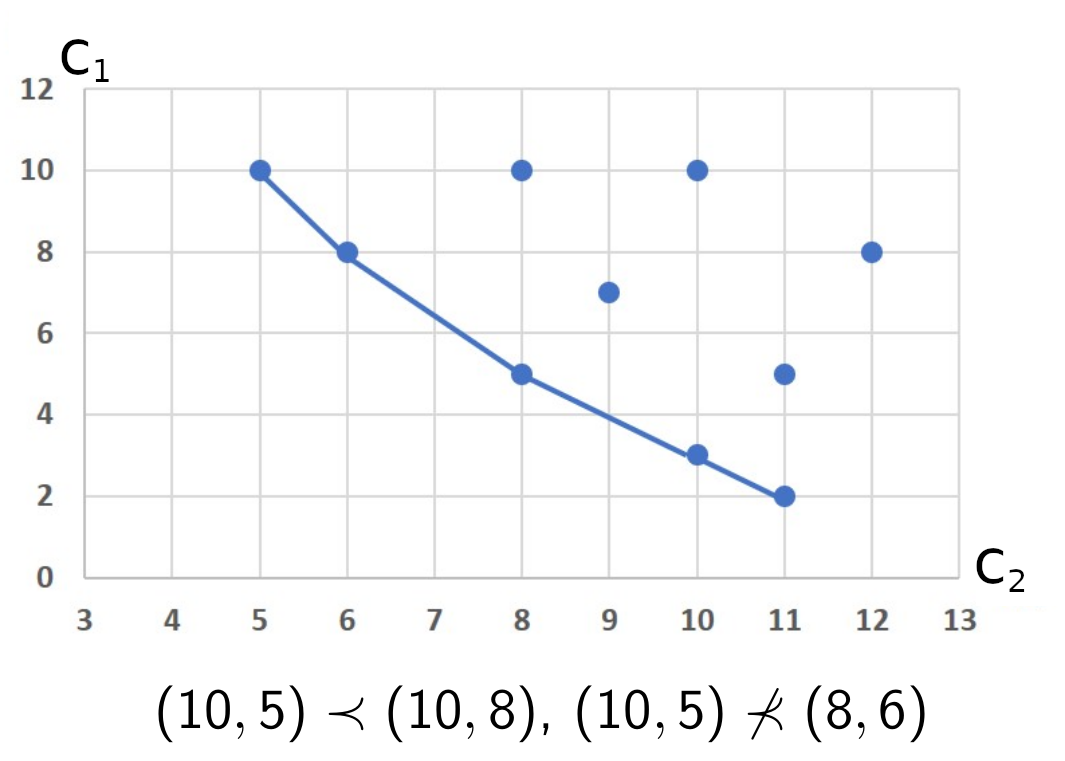
\includegraphics[scale=0.25]{domination}}}
\end{picture}

\end{frame}

\begin{frame}
\frametitle{Общий подход к решению бикритериальной задачи}
$OPEN$:
\begin{itemize}
\item $OPEN$ содержит нераскрытые узлы --- кортежи $x = (s, g, f)$, где $g$ и $f$ -- векторы
\item Для состояния $s$ в $OPEN$ одновременно могут находится несколько узлов $(s, g_1, f_1)$ и $(s, g_2, f_2)$
\end{itemize}
Выбор узла из $OPEN$:
\begin{itemize}
\item Для раскрытия выбирается такой узел $(s, g, f) \in OPEN$, что $\nexists (s ^ {'}, g ^ {'}, f ^ {'}) \in OPEN: f ^ {'} \prec f$ \\
Для бикритериальной задачи это условие эквивалентно извлечению узла с лексикографически минимальным значением $f$
\end{itemize}
Обработка узлов вида $(s_{goal}, g, f)$:
\begin{itemize}
\item Поддерживается множество найденный решений: $SOL = \{\pi_i (s_{start}, s_{goal})\}$
\item Если для найденного маршрута $\pi(s_{start}, s_{goal}) \Rightarrow \nexists \pi ^ {'} \in SOL: \pi ^ {'} \prec \pi$, то удаляем из $SOL$ все маршруты $\tilde{\pi}: \pi \prec \tilde{\pi}$ и добавляем $\pi$ в $SOL$
\end{itemize}
Раскрытие узла $(s, g, f)$:
\begin{itemize}
\item Для каждого дочернего состояния $s ^ {'} \in Succ(s)$ строится узел $(s ^ {'}, g ^ {'}, f ^ {'})$
\item Дочерний узел $(s ^ {'}, g ^ {'}, f ^ {'})$ добавляется в $OPEN$ при одновременном выполнении двух условий:
\begin{itemize}
\item $\nexists (s ^ {'}, \tilde{g}, \tilde{f}) \in OPEN: \tilde{f} \prec f ^ {'}$
\item $\nexists \pi \in SOL: \mathbb{c}(\pi) \prec f ^ {'}$
\end{itemize}
\item Если $(s ^ {'}, g ^ {'}, f ^ {'})$ добавляется в $OPEN$, то из $OPEN$ удаляются все узлы $(s ^ {'}, \tilde{g}, \tilde{f}): f ^ {'} \prec \tilde{f}$
\end{itemize}
Если $OPEN$ пустой, то алгоритм завершает работу и возвращает $SOL$.

\end{frame}

\begin{frame}
\frametitle{Алгоритмы}
Алгоритм NAMOA*:
\begin{itemize}
\item Реализация общего подхода с незначительными оптимизациями за счёт поддержки множества всех раскрытых узлов $G_{cl}(s)$
\end{itemize}
\ \\ \ \\
Алгоритм NAMOA*dr
\begin{itemize}
\item Оптимизация операции добавления дочернего узла в $OPEN$ для случая монотонной эвристической функции и извлечения узлов из $OPEN$ в лексикографическом порядке по $f$:
\begin{itemize}
\item Проверка $\nexists \pi \in SOL: \mathbb{c}(\pi) \prec (f_1 ^ {'}, f_2 ^ {'})$ заменяется на $\min_{\pi \in SOL} {c_2(\pi)} \geq f_2 ^ {'}$
\item В некоторых случаях проверку $\nexists (s ^ {'}, \tilde{g}, \tilde{f}) \in OPEN: \tilde{f} \prec f ^ {'}$ можно можно заменить на $\min_{\tilde{f} \in OPEN} {\tilde{f}_2} \geq f_2 ^ {'}$
\end{itemize} 
\end{itemize}
\ \\ \ \\
Алгоритм BOA*:
\begin{itemize}
\item Для случая монотонной эвристической функции и извлечения узлов из $OPEN$ в лексикографическом порядке по $f$ доказаны ещё более сильные утверждения, которые позволяют все проверки доминирования совершать за константное время за счёт поддержки $g_2 ^ {min} (s)$ --- минимального значения $g_2$ для раскрытых узлов с состоянием $s$
\item В узлах дополнительно хранятся ссылки на родительские узлы: $x = (s, g, f, parent(x))$
\end{itemize}
\ \\ \ \\ \ \\
\footnotesize{Mandow, L., and Pérez-de-la-Cruz, J. (2010). Multiobjective A* search with consistent heuristics}\\
\footnotesize{Machuca, E., and Mandow, L. (2012). Multiobjective heuristic search in road maps}\\
\footnotesize{Hernández Ulloa, C., Yeoh, W., Baier, J. A., Zhang, H., Suazo, L., \& Koenig, S. (2020). A Simple and Fast Bi-Objective Search Algorithm}

\end{frame}

\begin{frame}
\frametitle{Bi-Objective A* (BOA*)}
Сравнение качества работы алгоритмов на дорожных картах городов США \\
9th DIMACS Implementation Challenge - Shortest Paths. Критерии --- длинна \\
маршрута и время движения по маршруту:
\begin{itemize}
\item NAMOA*, NAMOA*dr, BOA* --- авторские реализации (язык Си)
\item sBOA* --- модификация BOA* без применения оптимизаций, приводящих \\
к константному времени проверки условий доминирования, авторская \\
реализация (язык Си)
\item Оригинальные реализации на Си для Bi-Objective Dijkstra (BDijkstra) \\
и Bidirectional Bi-Objective Dijkstra (BBDijkstra) предоставлены авторами \\
этих алгоритмов
\end{itemize}

\begin{picture}(20, 20)
\put(0, -105){\hbox{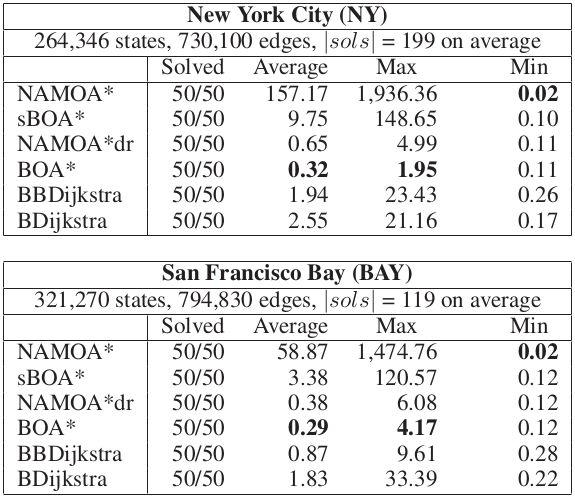
\includegraphics[scale=0.215]{results1}}}
\end{picture}

\begin{picture}(20, 20)
\put(130, -84){\hbox{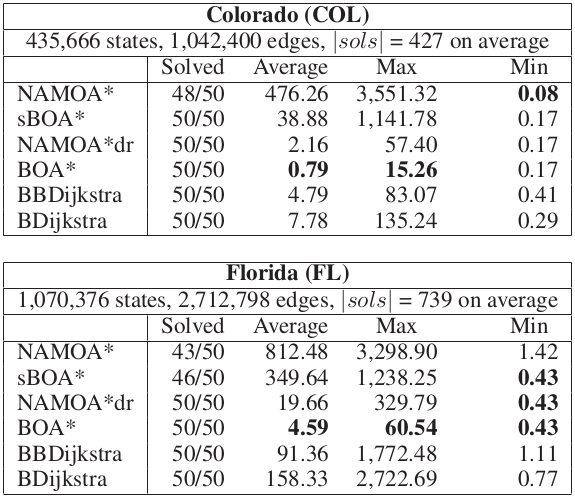
\includegraphics[scale=0.215]{results2}}}
\end{picture}

\begin{picture}(20, 20)
\put(300, -64){\hbox{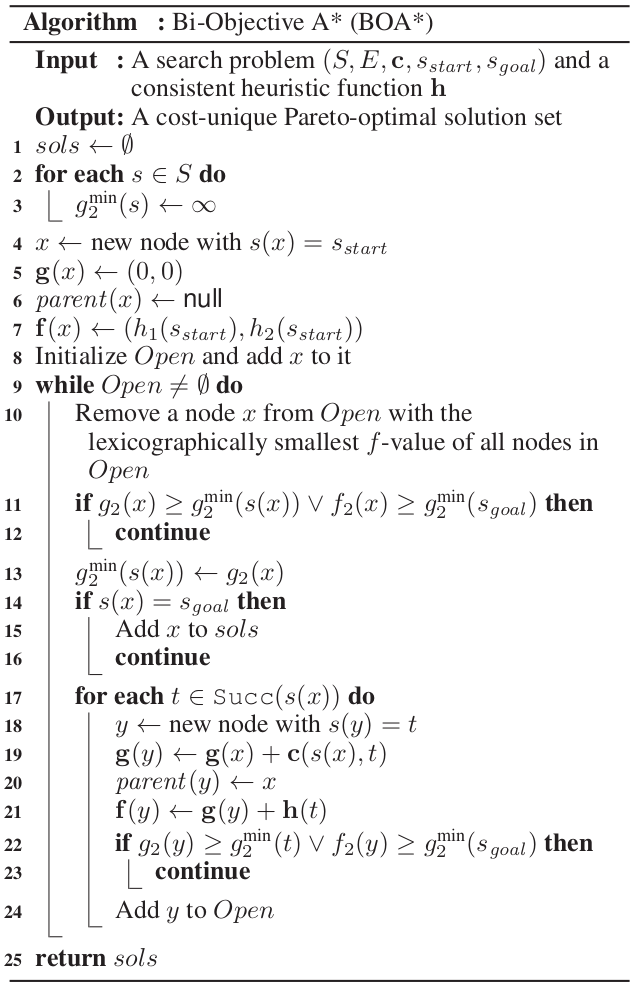
\includegraphics[scale=0.22]{boa}}}
\end{picture}
\ \\ \ \\ \ \\ \ \\ \ \\ \ \\ \ \\ \ \\

\end{frame}



\begin{frame}
\frametitle{План работы}
Репозиторий проекта: \url{https://github.com/ugadiarov-la-phystech-edu/hs-project}\\ \ \\
\begin{enumerate}
\item Набор данных для задачи бикритериальной оптимизации --- 9th DIMACS Implementation Challenge - Shortest Paths:
\begin{itemize}
\item \url{http://www.diag.uniroma1.it/challenge9/download.shtml}
\end{itemize}
\ \\ \ \\
\item Формирование размеченной выборки для проверки корректности реализуемых алгоритмов поиска множества парето-оптимальных решений:
\begin{itemize}
\item Использование алгоритма Дейкстры для поиска множества кротчайших путей по каждому критерию между парами вершин (пакет NetworkX: \url{https://networkx.org/})
\item Построение множества парето-оптимальных решений по результатам работы алгоритма Дейкстры
\end{itemize}
\ \\ \ \\
\item Реализация BOA*:
\begin{itemize}
\item Проверка корректности реализации на размеченной выборке
\item Эксперименты для оценки эффективности реализации: количество порождённых узлов, время работы
\item Оформление результатов
\end{itemize}
Срок: 26.04.2021
\ \\ \ \\
\item Реализация NAMOA*:
\begin{itemize}
\item Проверка корректности реализации на размеченной выборке
\item Эксперименты для оценки эффективности реализации: количество порождённых узлов, время работы
\item Оформление результатов
\end{itemize}
Срок: 03.05.2021
\end{enumerate}
\end{frame}


\end{document}
